\documentclass[11pt,pdf,ngerman,UKenglish]{beamer}%,handout
\usepackage[UKenglish]{babel}
\usepackage{array}
\usepackage[utf8]{inputenc}
\usepackage{amssymb}
\usepackage{amsmath}
%%\usepackage{amsfonts}
%%\usepackage{amstext}
\usepackage{amsthm}
%\usepackage{stmaryrd}
\usepackage{relsize}
%\usepackage{graphics}
\usepackage{graphicx}
%\usepackage{mathptmx}
%\usepackage[scaled]{uarial}
\usepackage[T1]{fontenc}
%%\usepackage{a4wide}
\usepackage{makeidx}
\usepackage{textcomp}
\usepackage{ulem}
\usepackage{geometry}
%\usepackage{bbm}
\usepackage{tikz}
\usepackage{hyperref}
\usepackage{sverb}
\usepackage{caption}
\usepackage{listings}
\usepackage{tabularx, multirow}
%\usepackage{booktabs}
%\usepackage{txfonts}
%\usepackage[ansinew]{inputenc}
%\usepackage[latin1]{inputenc}
\usepackage{enumerate}
\usepackage{bbold}
\usepackage{dsfont}
\usepackage{listings}
\usepackage{xifthen}

\usepackage{tikz}
\usepackage{pgfplots}
\pgfplotsset{compat=1.11}
\usepackage{xcolor}
\usepackage{subfigure}

\usepackage{epsdice}


\lstset{
	language=Matlab,% choose the language of the code
	basicstyle=\footnotesize,% the size of the fonts that are used for the code
	numbers=left,% where to put the line-numbers
	numberstyle=\scriptsize,% the size of the fonts that are used for the line-numbers
	stepnumber=1,% the step between two line-numbers. If it's 1 each line will be numbered
	numbersep=5pt,% how far the line-numbers are from the code
	%backgroundcolor=\color{white},% choose the background color. You must add \usepackage{color}
	showspaces=false,% show spaces adding particular underscores
	showstringspaces=false,% underline spaces within strings
	showtabs=false,% show tabs within strings adding particular underscores
	%frame=single,% adds a frame around the code
	%tabsize=2,% sets default tabsize to 2 spaces
	captionpos=t,% sets the caption-position to bottom
	%caption=\lstname,
	breaklines=false,% sets automatic line breaking
	breakatwhitespace=false,% sets if automatic breaks should only happen at whitespace
	escapeinside={\%*}{*)}% if you want to add a comment within your code
}
%%%%%%%%%%%%%%%%%%%%%%%%%%%%%%%%%%%%%%%%%%%%%%%%%%%%%%%

\newcommand{\IR}{\mathds{R}}
%\newcommand{\IN}{{\mathbb{N}}}
\newcommand{\IN}{\mathds{N}}
\newcommand{\IZ}{{\mathbb{Z}}}
\newcommand{\IF}{{\mathbb{F}}}
\newcommand{\IK}{{\mathbb{K}}}
\newcommand{\IQ}{{\mathbb{Q}}}
\newcommand{\IC}{{\mathbb{C}}}
%\newcommand{\IP}{{\mathbb{P}}}
\newcommand{\IP}{\mathbb{P}}
\newcommand{\IE}{{\mathbb{E}}}
%\newcommand{\E}{\mbox{I\negthinspace E}}% Zeichen für den Erwartungswert
\newcommand{\E}{\mathds{E}}
\newcommand{\F}{\mathcal{F}}
\renewcommand{\S}{\mathcal{S}}

\newcommand{\de}{\delta}
\newcommand{\vol}{\operatorname{vol}}
\newcommand{\sk}{{\,|\,}}
\newcommand{\arccot}{\operatorname{arccot}}
\newcommand{\1}{\mathbb{1}}
\newcommand{\supp}{\operatorname{supp}}
\renewcommand{\phi}{\varphi}
\renewcommand{\epsilon}{\varepsilon}
\renewcommand{\Re}{\operatorname{Re}}
\newcommand{\aeq}{\Leftrightarrow}
%\newcommand{\M}{\widetilde{\text{M}}}
\newcommand{\erfc}{\operatorname{Erfc}}
\newcommand{\erf}{\operatorname{Erf}}
\newcommand{\qvar}[2]{\langle #1 , #1 \rangle _{#2}}
%\newcommand{\qvar}[2]{<\hspace{-1.5mm}#1\hspace{-0.3mm},\hspace{-0.5mm}#1\hspace{-1.5mm}>_{#2}}
\newcommand{\sign}{\operatorname{sign}}
\newcommand{\SEP}{\text{SEP}}
\newcommand{\M}{\mathcal{M}}
\newcommand{\conv}{\operatorname{conv}}

\newcommand{\Law}{\text{Law}}
 
\renewcommand{\qedsymbol}{$\blacksquare$}


\newcommand*{\cA}{\mathcal{A}}
\newcommand*{\cB}{\mathcal{B}}
\newcommand*{\cC}{\mathcal{C}}
\newcommand*{\cD}{\mathcal{D}}
\newcommand*{\cE}{\mathcal{E}}
\newcommand*{\cF}{\mathcal{F}}
\newcommand*{\cG}{\mathcal{G}}
\newcommand*{\cH}{\mathcal{H}}
\newcommand*{\cI}{\mathcal{I}}
\newcommand*{\cJ}{\mathcal{J}}
\newcommand*{\cK}{\mathcal{K}}
\newcommand*{\cL}{\mathcal{L}}
\newcommand*{\cM}{\mathcal{M}}
\newcommand*{\cN}{\mathcal{N}}
\newcommand*{\cO}{\mathcal{O}}
\newcommand*{\cP}{\mathcal{P}}
\newcommand*{\cQ}{\mathcal{Q}}
\newcommand*{\cR}{\mathcal{R}}
\newcommand*{\cS}{\mathcal{S}}
\newcommand*{\cT}{\mathcal{T}}
\newcommand*{\cU}{\mathcal{U}}
\newcommand*{\cX}{\mathcal{X}}
\newcommand*{\cY}{\mathcal{Y}}

\renewcommand{\d}{\operatorname{d} \hspace{-0.5mm}}
\newcommand{\Dt}{\operatorname{D}^t}
\newcommand{\Dw}{\operatorname{D}^w}
\newcommand{\diff}[3][]{\ifthenelse{\isempty{#1}}{#3_{#2}}{#3_{#1 #2}}}
%\newcommand{\diff}[3][]{\ifthenelse{\isempty{#1}}{\partial_{#2} #3}{\partial_{#1} \partial_{#2} #3}}

\newcommand{\p}[3]{#1^{(#2)}_{#3}}
\newcommand{\Xz}[2]{X^{(2), (#1) }_{ #2 }}
\newcommand{\Xd}[2]{X^{(3), (#1) }_{ #2 }}
\newcommand{\dx}[1]{\frac{\d}{\d x^{(#1)}}}
\newcommand{\X}[2]{\p{X}{#1}{#2}}%{X^{(#1)}_{#2}}
\newcommand{\x}[1]{x^{(#1)}}
\renewcommand{\u}[2]{\ifthenelse{\isempty{#2}}{u^{(#1)}}{u^{(#1)}_{#2}}} %\p{u}{#1}{#2}}
\newcommand{\ut}[2]{\p{\tilde{u}}{#1}{#2}}%{\tilde{u}^{(#1)}_{#2}}
\newcommand{\Z}[2]{\p{\tilde{Z}}{#1}{#2}}%{\tilde{Z}^{(#1)}_{#2}}
\newcommand{\Zo}[2]{\p{Z}{#1}{#2}}%{Z^{(#1)}_{#2}}
\newcommand{\W}[1]{\widetilde{W}_{#1}}
\newcommand{\Y}[2]{\p{Y}{#1}{#2}}%{Y^{(#1)}_{#2}}
\newcommand{\Zh}[1]{\hat{Z}_{#1}}

\newcommand{\myitem}{$\bullet$\hspace*{-3mm}}

\newcommand{\Ito}{It\^o\ }
\newcommand{\Itos}{It\^o's\ }


\newtheoremstyle{thm}% name
{10pt}% Space above
{18pt}% Space below 
{\itshape}% Body font
{}% Indent amount: Indent amount: empty = no indent, \parindent = normal paragraph indent
{\bf}% Theorem head font
{}% Punctuation after theorem head
{\newline }% Space after theorem head: { } = normal interword space; \newline = linebreak
{}% Theorem head spec (can be left empty, meaning `normal')

\newtheoremstyle{def}% name
{10pt}% Space above
{18pt}% Space below 
{}% Body font
{}% Indent amount: Indent amount: empty = no indent, \parindent = normal paragraph indent
{\bf}% Theorem head font
{}% Punctuation after theorem head
{\newline }% Space after theorem head: { } = normal interword space; \newline = linebreak
{}% Theorem head spec (can be left empty, meaning `normal')


\theoremstyle{thm}

%\newtheorem{theorem}{Theorem}[section]
%\newtheorem{lemma}[theorem]{Lemma}
\newtheorem{proposition}[theorem]{Proposition}
%\newtheorem{corollary}[theorem]{Corollary}

\newtheorem{assumption}[theorem]{Assumption}
\newtheorem{algorithm}[theorem]{Algorithm}

\theoremstyle{def}
%\newtheorem{definition}[theorem]{Definition}
%\newtheorem{example}[theorem]{Example}
%\newtheorem{remarks}[theorem]{Remark}

\renewenvironment{proof}{\par\noindent\textit{Proof.~}}{\hfill \qedsymbol\newline}

 
 
 
%\newtheorem{satz}{Satz}
%\newtheorem{theorem}{Theorem}%[section]
%\newtheorem{lemma}[theorem]{Lemma}
%\newtheorem{proposition}[theorem]{Proposition}
%\newtheorem{corollary}[theorem]{Corollary}
%\newtheorem{remarks}{Bemerkung}
%\newtheorem{definition}{Definition}
%\newtheorem{example}{Beispiel}
%%%%%%%%%%%%%%%%%%%%%%%%%%%%%%%%%%%%%%%%%%%%%%%%%%%%%%%

%Madrid %Singapore %Copenhagen %Warsaw
\mode<presentation>{\usetheme{Frankfurt}}

\title{Probability}
\author{Stefan Engelhardt}
\date{3rd October 2023}%{\today}%{25st Jannuary 2022}
%\logo{...}

\setbeamercovered{transparent}

\begin{document}

\begin{frame}
\titlepage
\end{frame}
% Remove logo from the next slides
\logo{}



\begin{frame}{Random Variables}

\begin{block}{Definition: Random Variable}
A random variable is a {\color{gray}{measurable}} function on the sample space.
\end{block}
\ \\
Usually: $X: \Omega \to \IR$

\pause
\begin{align*}
\IP(X \leq x) 
\simeq & \text{"What is the probability that }X\text{ takes a value that is}
\\& \ \text{ smaller or equal to }x\text{?"}
\pause
\\
= & \IP(\{ \omega \in \Omega:\ X(\omega) \leq x \} )
.
\end{align*}
\end{frame}


\begin{frame}{Discrete Random Variable}
\begin{block}{Definition: Discrete Random Variable}
A random variable that can take on at most a countable number of possible values is called discrete.
\end{block}
\
\pause

Let $X$ be a discrete random variable and denote by $(x_i)_{i\in I}$ the sequence of all values $X$ can adopt.

\begin{block}{Definition: Probability Mass Function}
We call the function $p$ with $p(x_i) = \IP( X = x_i)$ for all $i$ the probability mass function of the random variable $X$.
\end{block}
\

Note that $\sum_{i \in I} p(x_i) = 1$.
\end{frame}


\begin{frame}{Binomial Distribution}
%Graph for n=5, p=1/2,    n=20, p=1/2
%          n=5, p=0.2,    n=5,  p=0.8
\vspace*{-9mm}
\begin{columns}[c]
    \column{0.4\textwidth}
        \begin{figure}
            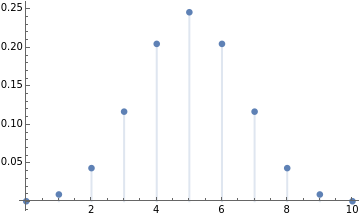
\includegraphics[scale=0.4]{BinomialPDF_10_05.png}
    	\caption{Bin(10, 0.5)}
        \end{figure}
\vspace*{-9mm}
        \begin{figure}
            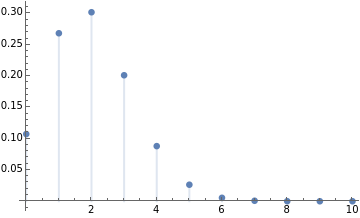
\includegraphics[scale=0.4]{BinomialPDF_10_02.png}
    	\caption{Bin(10, 0.2)}
        \end{figure}
    \column{0.4\textwidth}
        \begin{figure}
             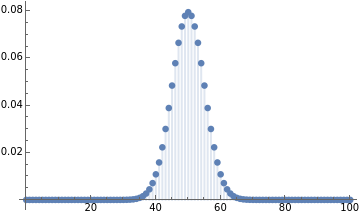
\includegraphics[scale=0.4]{BinomialPDF_100_05.png} 
    	\caption{Bin(100, 0.5)}
        \end{figure}
\vspace*{-9mm}
        \begin{figure}
            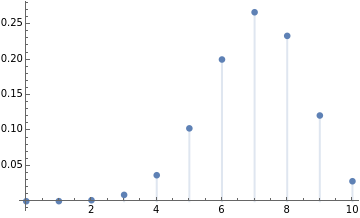
\includegraphics[scale=0.4]{BinomialPDF_10_07.png}
    	\caption{Bin(10, 0.7)}
        \end{figure}
\end{columns}
\end{frame}


\begin{frame}{Geometric Distribution}
\begin{block}{Definition: Geometric Distribution}
We call a random variable $X$ geometrically distributed to the parameter $p \in (0,1)$ if
$$ \IP(X=k)= (1-p)^{k-1}p, \quad \text{for all } k \in \{ 1,2,\ldots \}.$$
In this case we write $X \sim Geom(p)$.
\end{block}
\

Examples:
\begin{itemize}
\item Rolling dice till the first '6'.
\item Doing an experiment till the first success.
\item Switching a device off and on again until it works.
\end{itemize}
\end{frame}


\begin{frame}{Continuous Distributions}
Motivation:
\begin{itemize}
\item Radioactive atoms spontaneously decay.
\item If the atom has not yet decayed, then the probability that it decays in the next short time $\Delta t$ is $\approx \lambda \Delta t$ for some constant $\lambda$.
\item It does not matter how long the atom is around.
\end{itemize}
\ \\ \ \\
Define the random variable $T$ as the time of decay from now on.

\ \\
\pause
Problem:
\begin{itemize}
\item $T$ takes all values in $[0,\infty)$.
\item What is the probability of $T=7.5$ exactly?
\end{itemize}
\end{frame}


\begin{frame}{Probability density function}
%Concept:
%$$ \IP( X \in [a,b]) = \int_a^b f_X(x) dx$$
\begin{block}{Definition: Continuous distribution and pdf}
We say that a random variable $X$ has a continuous distribution if there exits a function $f_X: \IR \to \IR$ such that for any "nice" $B \subseteq \IR$
$$\IP(X \in B) = \int_B f_X(x) dx.$$
We call $f_X$ the probability density function (pdf) of X.
\end{block}
\
\begin{block}{Lemma}
Let $X$ be a continuous random variable and $f_X$ its pdf. Then
\begin{enumerate}
\item $f_X(x) \geq 0$ for all $x\in \IR$,
\item $\int_{-\infty}^\infty f_X(x) dx = 1$.
\end{enumerate}
\end{block}
\end{frame}


\begin{frame}{Cumulative distribution function}
\begin{block}{Definition: CDF}
For any random variable $X$ we define its cumulative distribution function (cdf) $F_X$ for all $x \in \IR$ by
$$ F_X(x) = \IP(X \leq x).$$
\end{block}
\
\begin{corollary}
For a continuous random variable $X$ with pdf $f_X$ we have that
$$ F_X(x) = \IP( X \leq x) = \IP( -\infty < X \leq x) = \int_{-\infty}^x f_X(y) dy.$$
\end{corollary}

\end{frame}


\begin{frame}
\begin{block}{Definition: CDF}
For any random variable $X$ we define its cumulative distribution function (cdf) $F_X$ for all $x \in \IR$ by
$$ F_X(x) = \IP(X \leq x).$$
\end{block}
\
\begin{proposition}
Let $X$ be a random variable.
\begin{itemize}
\item $F_X$ is non-decreasing.
\item $\lim_{x \searrow -\infty} F_X(x) = 0$ and $\lim_{x \nearrow \infty} F_X(x) = 1$.
\item If $X$ has a continuous distribution, then for all $x \in \IR$ where $f_X$ is continuous, $F_X$ is differentiable and $F_X'(x)=f_X(x)$.
\end{itemize}
\end{proposition}
\end{frame}

\end{document}
